% Drawing 70/03-2 -- folder 70, batch 03, archive page 52 (PDF page 53).
% Transcription: figure : le sommet $s_0$ d'où partent les arêtes $a_0$ (vers $s_1$), $a_1$ (vers $s_2$), $a_2$ (vers $s_3$, vers le haut) et une quatrième arête vers le bas, aboutissant à un point marqué $s_3$ (surchargé) ; les faces $f_0$ (entre $a_0$ et $a_1$, hachurée), $f_1$ (entre $a_2$ et $a_0$, hachurée), $f_2$ (sous $a_1$) et $f_3$ au-delà de $s_1$ ; une arête $a_2^0$ issue de $s_1$.
% Kind: vertex with edges and faces (flags). Method 2 (schematic redraw from the facsimile). Status: ok.
% Notes: Vertex s_0 with the edges a_0 (to s_1), a_1 (to s_2), a_2 (up) and a fourth edge down to a point marked s_3 (overwritten); faces f_1 (between a_2 and a_0, hatched by short strokes), f_0 (between a_0 and a_1, short hatching under a_0 and over a_1), f_2 (under a_1), f_3 beyond s_1 (hatched); from s_1 the edge a_2^0. Hatching drawn as short strokes as on the page.
% Coordinates: 1 unit = 1 mm = 1/100 of the crop width (bbox in page fractions: [0.08, 0.52, 0.42, 0.76]).
% Redrawn by Claude (claude-opus-5-5), issue #73, 2026-11-07; not checked by a human; not compiled (no TeX in the session).
% Rights: reproduces part of the work -- behind RENDER_TRANSCRIPTS, never published by itself.
\documentclass[tikz,border=3pt]{standalone}
\usepackage{amsmath,amssymb}
\usetikzlibrary{patterns,arrows.meta}
\tikzset{pencil/.style={black!45}, struck/.style={black!35}, mark/.style={circle,draw,inner sep=1.3pt}, pt/.style={circle,fill,inner sep=0.9pt}, opt/.style={circle,draw,fill=white,inner sep=1.1pt}}
\begin{document}
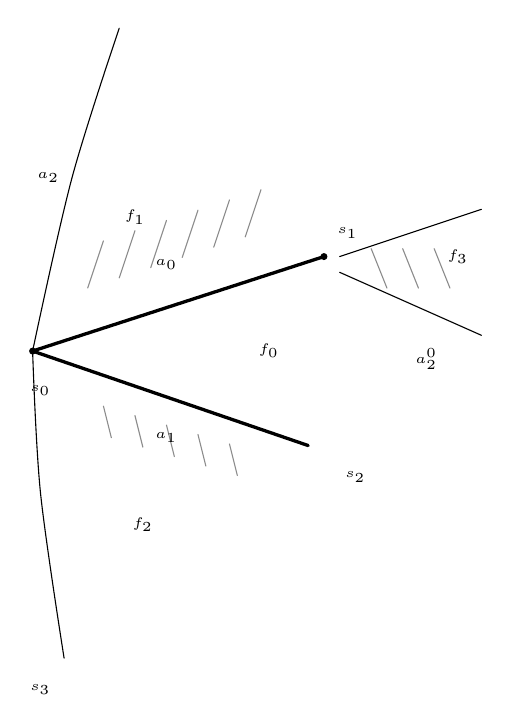
\begin{tikzpicture}[x=1mm,y=1mm,line cap=round,line join=round,font=\scriptsize]
\draw[very thick] (43,-42) -- (80,-30);
\draw[very thick] (43,-42) -- (78,-54);
\draw plot[smooth, tension=0.55] coordinates {(54,-1) (48,-20) (43,-42)};
\draw plot[smooth, tension=0.55] coordinates {(43,-42) (44,-60) (47,-81)};
\node[pt] at (43,-42) {};
\node[pt] at (80,-30) {};
\draw (82,-32) -- (100,-40);
\draw (82,-30) -- (100,-24);
\draw[pencil] (50,-34) -- (52,-28);
\draw[pencil] (54,-32.7) -- (56,-26.7);
\draw[pencil] (58,-31.4) -- (60,-25.4);
\draw[pencil] (62,-30.1) -- (64,-24.1);
\draw[pencil] (66,-28.8) -- (68,-22.8);
\draw[pencil] (70,-27.5) -- (72,-21.5);
\draw[pencil] (52,-49) -- (53,-53);
\draw[pencil] (56,-50.2) -- (57,-54.2);
\draw[pencil] (60,-51.4) -- (61,-55.4);
\draw[pencil] (64,-52.6) -- (65,-56.6);
\draw[pencil] (68,-53.8) -- (69,-57.8);
\draw[pencil] (86,-29) -- (88,-34);
\draw[pencil] (90,-29) -- (92,-34);
\draw[pencil] (94,-29) -- (96,-34);
\node[inner sep=1pt] at (44,-47) {\tiny $s_0$};
\node[inner sep=1pt] at (83,-27) {\tiny $s_1$};
\node[inner sep=1pt] at (84,-58) {\tiny $s_2$};
\node[inner sep=1pt] at (44,-85) {\tiny $s_3$};
\node[inner sep=1pt] at (60,-31) {\tiny $a_0$};
\node[inner sep=1pt] at (60,-53) {\tiny $a_1$};
\node[inner sep=1pt] at (45,-20) {\tiny $a_2$};
\node[inner sep=1pt] at (93,-43) {\tiny $a_2^0$};
\node[inner sep=1pt] at (56,-25) {\tiny $f_1$};
\node[inner sep=1pt] at (73,-42) {\tiny $f_0$};
\node[inner sep=1pt] at (57,-64) {\tiny $f_2$};
\node[inner sep=1pt] at (97,-30) {\tiny $f_3$};
\end{tikzpicture}
\end{document}
